%------------------------------------------------------------------------------
\section{Outline}
{\large MATZO BALLS!}
\begin{itemize}
\item Autonomous vehicles are awesome blurb 

\item Big challenge in verifying the vehicle's operation between the levels of behavioral planning and trajectory tracking, inclusive. 
\item Source of challenge: variations in physical environment (road networks and regulations), variations in other vehicles (number and behavior), errors of ego vehicle state estimation, imperfect plan execution.
\item We present three benchmarks, which we call scenarios, and preliminary experience in running dReach to verify them.
\item Why reachability rather than, say, stochastic simulation?
\item Ego vehicle model: given a reference trajectory, bicycle model ODE. Environment mode contains reference trajectories for the center of the lane. 
\item Reference trajectory is generated by pure pursuit. 
\item Target point for pure pursuit is generated by hybrid automaton behavioral planner.
\item Other vehicle models
\item Scenario 1: 2 cars on straight road, lane changing.
Describe road network, agents, properties to be satisfied, one dReach run on it.
dReach run results include time bound on verification, tool runtime, number of jumps, number of time steps/jump (?)
\item Scenario 2: 3 cars on curved road. 
Describe same as above.
Then describe 3 successively more complex configurations of that same scenario, but in less detail.
\item Scenario 3: General description of traffic light. Highlight the need for composable agent models. Can no longer hand design verification instance. 
\item Extensions of benchmarks: what can be added to the models to make them more realistic?
\end{itemize}

%------------------------------------------------------------------------------
\section{Introduction}
\label{sect:introduction}

\begin{itemize}
	\item NHTSB says AV software is considered a driver. How does one bound the risk posed to society by software agent. 
	\item Driver's license is a set of tests, we attempt to generalize human behavior based on tests
	\item AV's don't necessarily fail in predictable ways, tests cover an infitesimal portion of the state space, need to gain confidence that algorithms are sound.
	\item Verification Methods and Tools
	\begin{itemize}
		\item Industry Perspective: Testing and Simulation
		\item Control Perspective: Lyapunov Functions
		\item Software Perspective: Model Checking
		\item Logic Perspective: Theorem Proving
	\end{itemize}
\end{itemize}
CPS perspective is an integrated approach that captures the manifestation of errors in the physical world. At its heart is the use of formal models of system and precise mathematical specifications of desired behavior. We are interested in developing the appropriate formal models, a set of specifications, and a battery of scenarios. The community needs to investigate how such methods scale, or fail to scale, and provide new solutions.

\begin{figure}
	\centering
	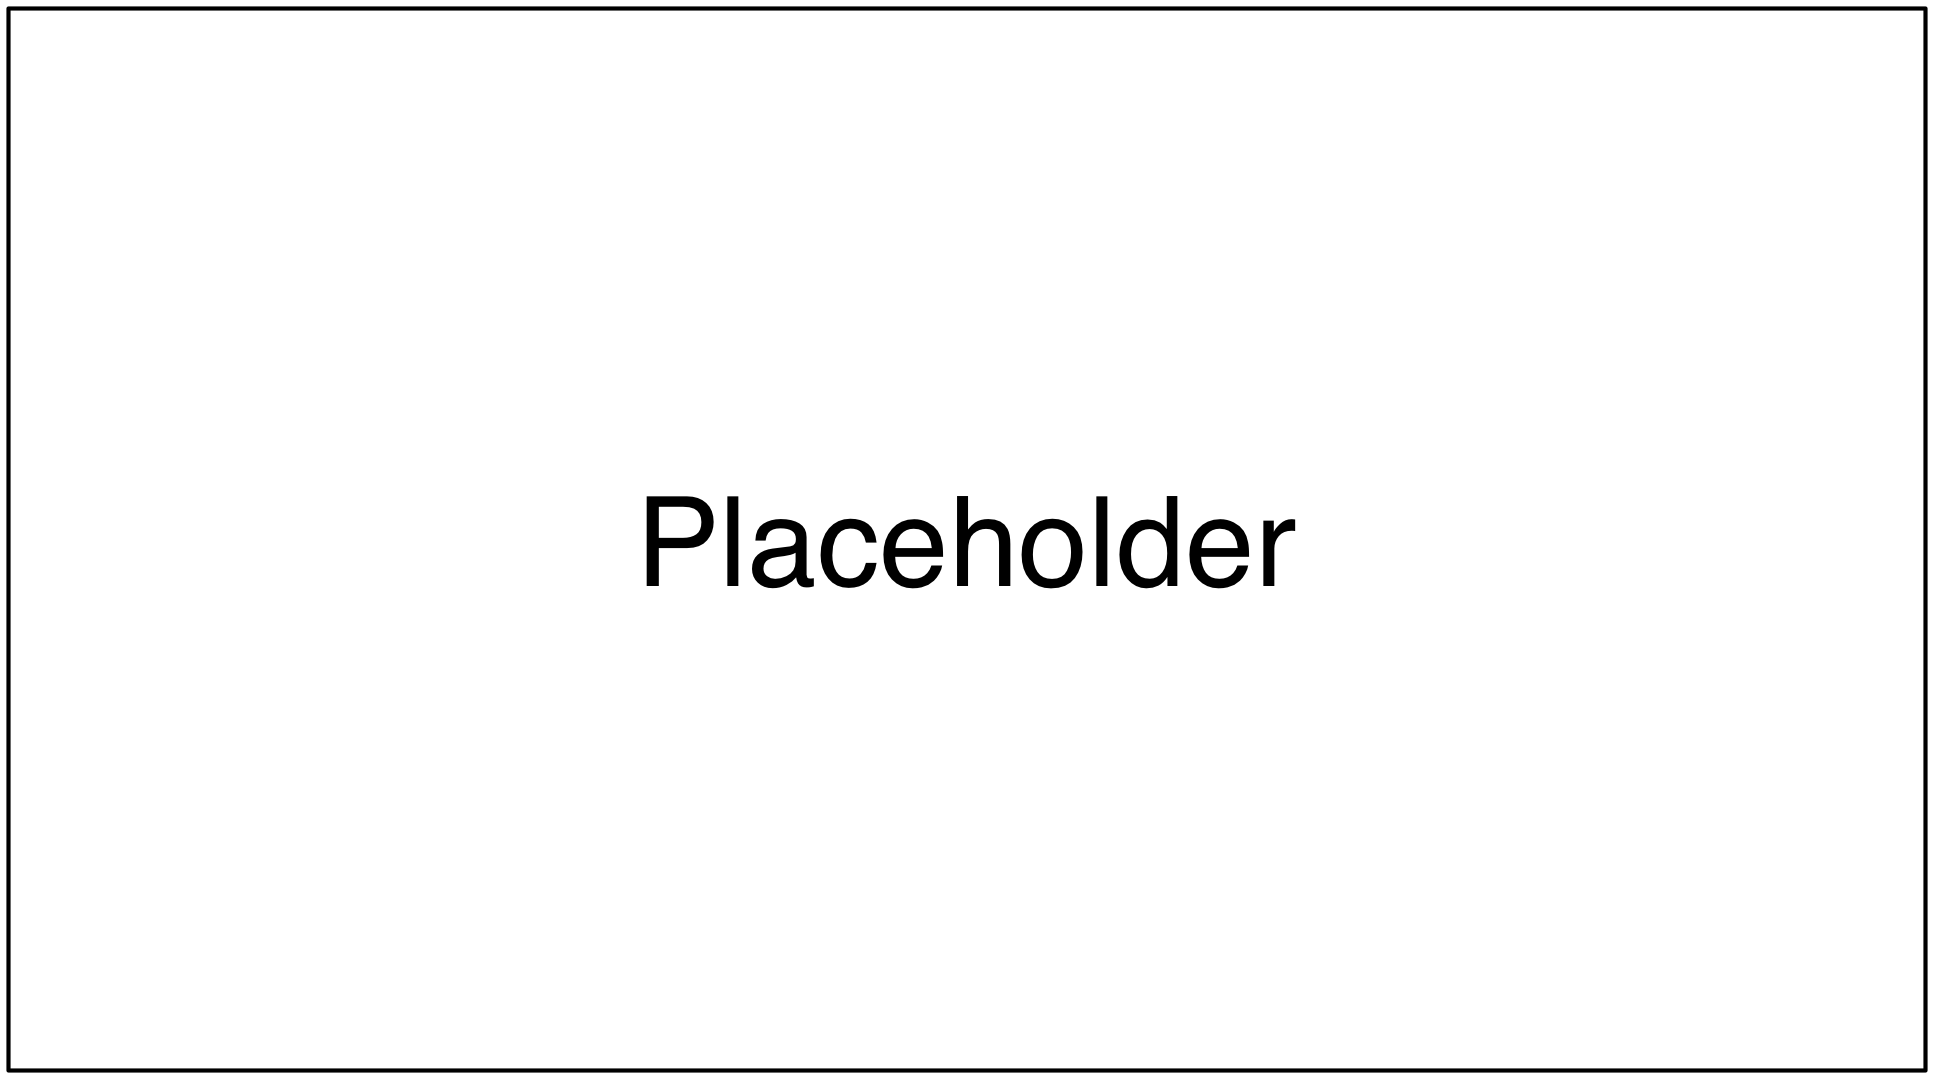
\includegraphics[scale=0.5]{figures/placeholder}
	\caption{A grid of canonical driving scenarios which a human driver might encounter in a certification procedure, highlighted, scenarios covered in this benchmark set}
\end{figure}
